\documentclass[1p]{elsarticle_modified}
%\bibliographystyle{elsarticle-num}

%\usepackage[colorlinks]{hyperref}
%\usepackage{abbrmath_seonhwa} %\Abb, \Ascr, \Acal ,\Abf, \Afrak
\usepackage{amsfonts}
\usepackage{amssymb}
\usepackage{amsmath}
\usepackage{amsthm}
\usepackage{scalefnt}
\usepackage{amsbsy}
\usepackage{kotex}
\usepackage{caption}
\usepackage{subfig}
\usepackage{color}
\usepackage{graphicx}
\usepackage{xcolor} %% white, black, red, green, blue, cyan, magenta, yellow
\usepackage{float}
\usepackage{setspace}
\usepackage{hyperref}

\usepackage{tikz}
\usetikzlibrary{arrows}

\usepackage{multirow}
\usepackage{array} % fixed length table
\usepackage{hhline}

%%%%%%%%%%%%%%%%%%%%%
\makeatletter
\renewcommand*\env@matrix[1][\arraystretch]{%
	\edef\arraystretch{#1}%
	\hskip -\arraycolsep
	\let\@ifnextchar\new@ifnextchar
	\array{*\c@MaxMatrixCols c}}
\makeatother %https://tex.stackexchange.com/questions/14071/how-can-i-increase-the-line-spacing-in-a-matrix
%%%%%%%%%%%%%%%

\usepackage[normalem]{ulem}

\newcommand{\msout}[1]{\ifmmode\text{\sout{\ensuremath{#1}}}\else\sout{#1}\fi}
%SOURCE: \msout is \stkout macro in https://tex.stackexchange.com/questions/20609/strikeout-in-math-mode

\newcommand{\cancel}[1]{
	\ifmmode
	{\color{red}\msout{#1}}
	\else
	{\color{red}\sout{#1}}
	\fi
}

\newcommand{\add}[1]{
	{\color{blue}\uwave{#1}}
}

\newcommand{\replace}[2]{
	\ifmmode
	{\color{red}\msout{#1}}{\color{blue}\uwave{#2}}
	\else
	{\color{red}\sout{#1}}{\color{blue}\uwave{#2}}
	\fi
}

\newcommand{\Sol}{\mathcal{S}} %segment
\newcommand{\D}{D} %diagram
\newcommand{\A}{\mathcal{A}} %arc


%%%%%%%%%%%%%%%%%%%%%%%%%%%%%5 test

\def\sl{\operatorname{\textup{SL}}(2,\Cbb)}
\def\psl{\operatorname{\textup{PSL}}(2,\Cbb)}
\def\quan{\mkern 1mu \triangleright \mkern 1mu}

\theoremstyle{definition}
\newtheorem{thm}{Theorem}[section]
\newtheorem{prop}[thm]{Proposition}
\newtheorem{lem}[thm]{Lemma}
\newtheorem{ques}[thm]{Question}
\newtheorem{cor}[thm]{Corollary}
\newtheorem{defn}[thm]{Definition}
\newtheorem{exam}[thm]{Example}
\newtheorem{rmk}[thm]{Remark}
\newtheorem{alg}[thm]{Algorithm}

\newcommand{\I}{\sqrt{-1}}
\begin{document}

%\begin{frontmatter}
%
%\title{Boundary parabolic representations of knots up to 8 crossings}
%
%%% Group authors per affiliation:
%\author{Yunhi Cho} 
%\address{Department of Mathematics, University of Seoul, Seoul, Korea}
%\ead{yhcho@uos.ac.kr}
%
%
%\author{Seonhwa Kim} %\fnref{s_kim}}
%\address{Center for Geometry and Physics, Institute for Basic Science, Pohang, 37673, Korea}
%\ead{ryeona17@ibs.re.kr}
%
%\author{Hyuk Kim}
%\address{Department of Mathematical Sciences, Seoul National University, Seoul 08826, Korea}
%\ead{hyukkim@snu.ac.kr}
%
%\author{Seokbeom Yoon}
%\address{Department of Mathematical Sciences, Seoul National University, Seoul, 08826,  Korea}
%\ead{sbyoon15@snu.ac.kr}
%
%\begin{abstract}
%We find all boundary parabolic representation of knots up to 8 crossings.
%
%\end{abstract}
%\begin{keyword}
%    \MSC[2010] 57M25 
%\end{keyword}
%
%\end{frontmatter}

%\linenumbers
%\tableofcontents
%
\newcommand\colored[1]{\textcolor{white}{\rule[-0.35ex]{0.8em}{1.4ex}}\kern-0.8em\color{red} #1}%
%\newcommand\colored[1]{\textcolor{white}{ #1}\kern-2.17ex	\textcolor{white}{ #1}\kern-1.81ex	\textcolor{white}{ #1}\kern-2.15ex\color{red}#1	}

{\Large $\underline{12a_{0752}~(K12a_{0752})}$}

\setlength{\tabcolsep}{10pt}
\renewcommand{\arraystretch}{1.6}
\vspace{1cm}\begin{tabular}{m{100pt}>{\centering\arraybackslash}m{274pt}}
\multirow{5}{120pt}{
	\centering
	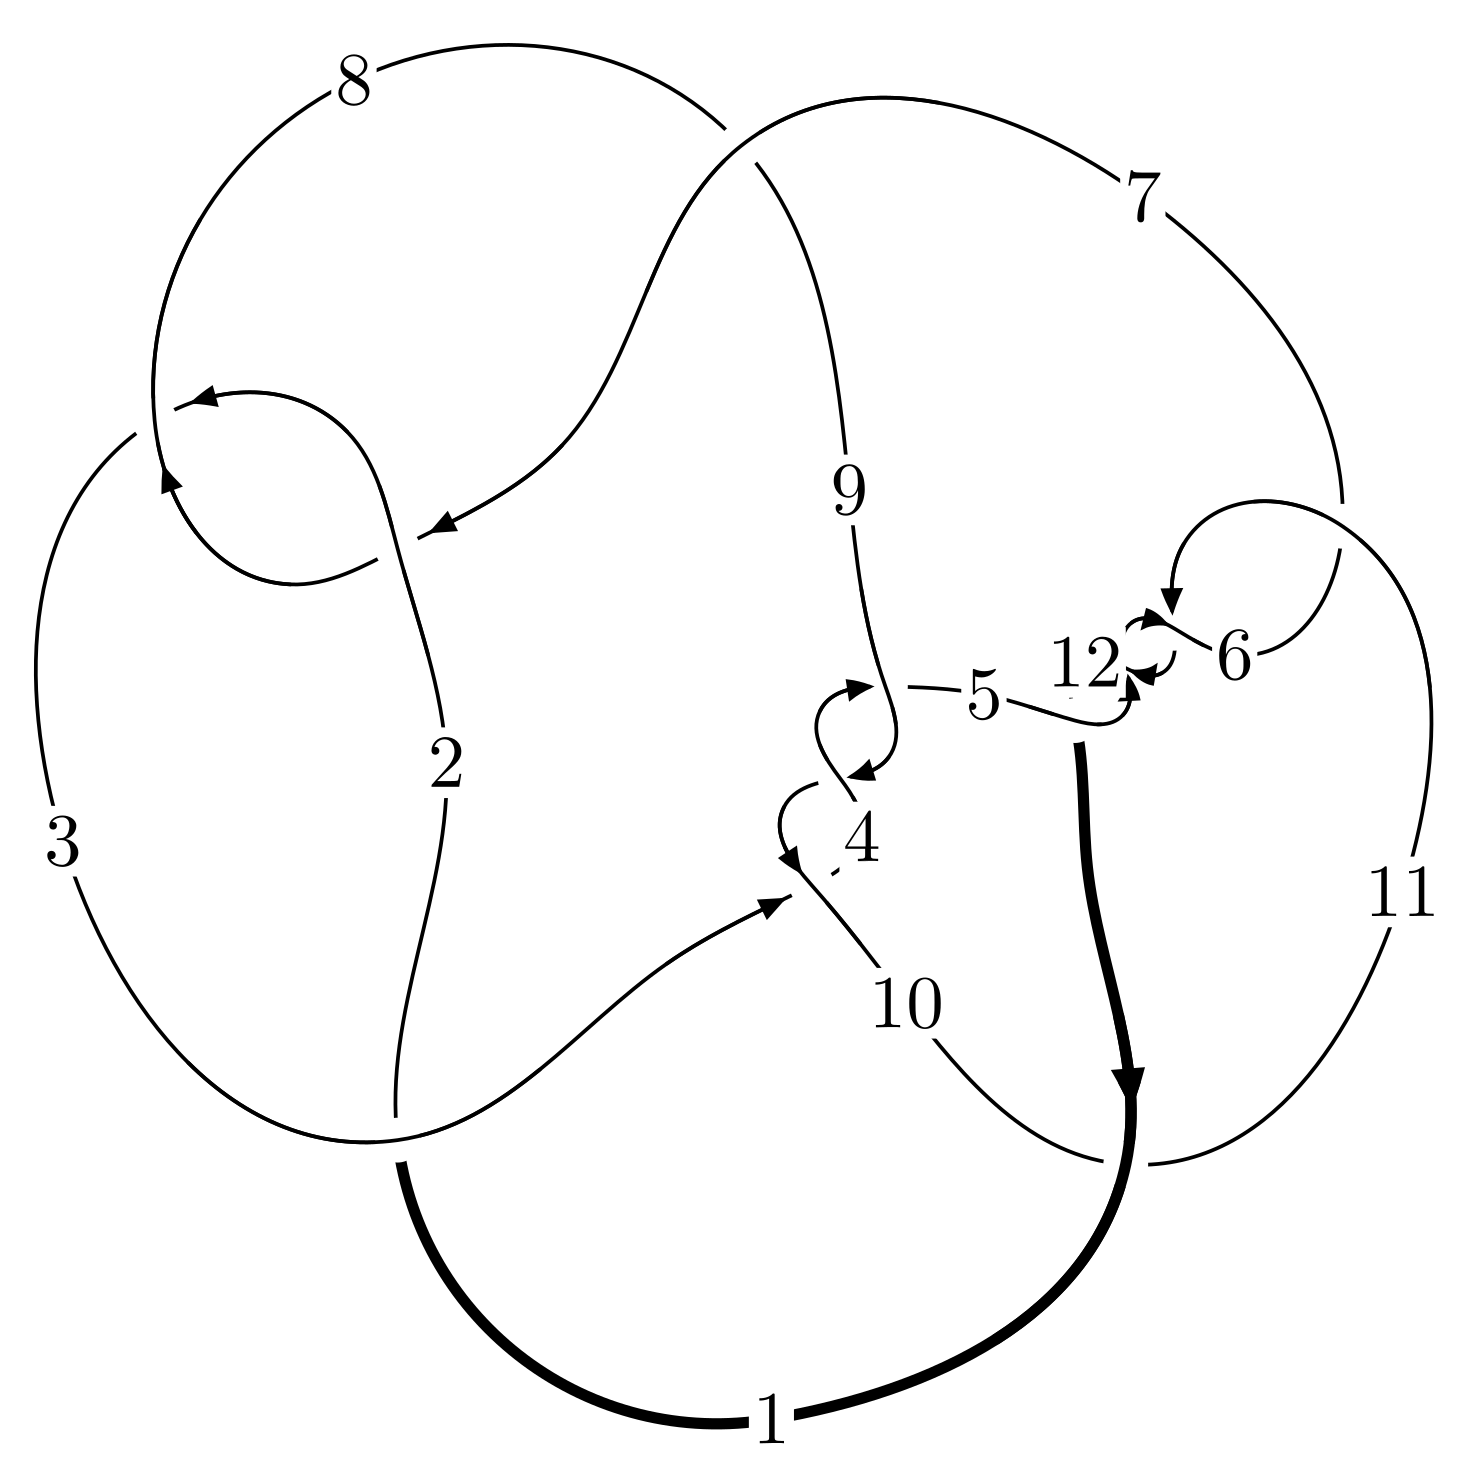
\includegraphics[width=112pt]{../../../GIT/diagram.site/Diagrams/png/1553_12a_0752.png}\\
\ \ \ A knot diagram\footnotemark}&
\allowdisplaybreaks
\textbf{Linearized knot diagam} \\
\cline{2-2}
 &
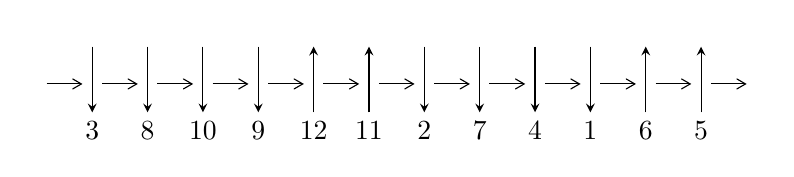
\begin{tikzpicture}[x=20pt, y=17pt]
	% nodes
	\node (C0) at (0, 0) {};
	\node (C1) at (1, 0) {};
	\node (C1U) at (1, +1) {};
	\node (C1D) at (1, -1) {3};

	\node (C2) at (2, 0) {};
	\node (C2U) at (2, +1) {};
	\node (C2D) at (2, -1) {8};

	\node (C3) at (3, 0) {};
	\node (C3U) at (3, +1) {};
	\node (C3D) at (3, -1) {10};

	\node (C4) at (4, 0) {};
	\node (C4U) at (4, +1) {};
	\node (C4D) at (4, -1) {9};

	\node (C5) at (5, 0) {};
	\node (C5U) at (5, +1) {};
	\node (C5D) at (5, -1) {12};

	\node (C6) at (6, 0) {};
	\node (C6U) at (6, +1) {};
	\node (C6D) at (6, -1) {11};

	\node (C7) at (7, 0) {};
	\node (C7U) at (7, +1) {};
	\node (C7D) at (7, -1) {2};

	\node (C8) at (8, 0) {};
	\node (C8U) at (8, +1) {};
	\node (C8D) at (8, -1) {7};

	\node (C9) at (9, 0) {};
	\node (C9U) at (9, +1) {};
	\node (C9D) at (9, -1) {4};

	\node (C10) at (10, 0) {};
	\node (C10U) at (10, +1) {};
	\node (C10D) at (10, -1) {1};

	\node (C11) at (11, 0) {};
	\node (C11U) at (11, +1) {};
	\node (C11D) at (11, -1) {6};

	\node (C12) at (12, 0) {};
	\node (C12U) at (12, +1) {};
	\node (C12D) at (12, -1) {5};
	\node (C13) at (13, 0) {};

	% arrows
	\draw[->,>={angle 60}]
	(C0) edge (C1) (C1) edge (C2) (C2) edge (C3) (C3) edge (C4) (C4) edge (C5) (C5) edge (C6) (C6) edge (C7) (C7) edge (C8) (C8) edge (C9) (C9) edge (C10) (C10) edge (C11) (C11) edge (C12) (C12) edge (C13) ;	\draw[->,>=stealth]
	(C1U) edge (C1D) (C2U) edge (C2D) (C3U) edge (C3D) (C4U) edge (C4D) (C5D) edge (C5U) (C6D) edge (C6U) (C7U) edge (C7D) (C8U) edge (C8D) (C9U) edge (C9D) (C10U) edge (C10D) (C11D) edge (C11U) (C12D) edge (C12U) ;
	\end{tikzpicture} \\
\hhline{~~} \\& 
\textbf{Solving Sequence} \\ \cline{2-2} 
 &
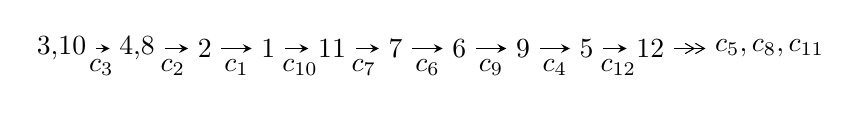
\begin{tikzpicture}[x=23pt, y=7pt]
	% node
	\node (A0) at (-1/8, 0) {3,10};
	\node (A1) at (17/16, 0) {4,8};
	\node (A2) at (17/8, 0) {2};
	\node (A3) at (25/8, 0) {1};
	\node (A4) at (33/8, 0) {11};
	\node (A5) at (41/8, 0) {7};
	\node (A6) at (49/8, 0) {6};
	\node (A7) at (57/8, 0) {9};
	\node (A8) at (65/8, 0) {5};
	\node (A9) at (73/8, 0) {12};
	\node (C1) at (1/2, -1) {$c_{3}$};
	\node (C2) at (13/8, -1) {$c_{2}$};
	\node (C3) at (21/8, -1) {$c_{1}$};
	\node (C4) at (29/8, -1) {$c_{10}$};
	\node (C5) at (37/8, -1) {$c_{7}$};
	\node (C6) at (45/8, -1) {$c_{6}$};
	\node (C7) at (53/8, -1) {$c_{9}$};
	\node (C8) at (61/8, -1) {$c_{4}$};
	\node (C9) at (69/8, -1) {$c_{12}$};
	\node (A10) at (11, 0) {$c_{5},c_{8},c_{11}$};

	% edge
	\draw[->,>=stealth]	
	(A0) edge (A1) (A1) edge (A2) (A2) edge (A3) (A3) edge (A4) (A4) edge (A5) (A5) edge (A6) (A6) edge (A7) (A7) edge (A8) (A8) edge (A9) ;
	\draw[->>,>={angle 60}]	
	(A9) edge (A10);
\end{tikzpicture} \\ 

\end{tabular} \\

\footnotetext{
The image of knot diagram is generated by the software ``\textbf{Draw programme}" developed by Andrew Bartholomew(\url{http://www.layer8.co.uk/maths/draw/index.htm\#Running-draw}), where we modified some parts for our purpose(\url{https://github.com/CATsTAILs/LinksPainter}).
}\phantom \\ \newline 
\centering \textbf{Ideals for irreducible components\footnotemark of $X_{\text{par}}$} 
 
\begin{align*}
I^u_{1}&=\langle 
9.34661\times10^{34} u^{64}-1.16625\times10^{35} u^{63}+\cdots+2.68953\times10^{35} b+2.48209\times10^{35},\\
\phantom{I^u_{1}}&\phantom{= \langle  }-2.45811\times10^{33} u^{64}+8.33232\times10^{33} u^{63}+\cdots+1.12064\times10^{34} a+2.26849\times10^{34},\;u^{65}- u^{64}+\cdots+12 u-4\rangle \\
I^u_{2}&=\langle 
- a^3 u-2 a^2 u-3 a^2+a u+2 b-4 a+3 u-1,\;a^4-4 a^3 u+a^3-3 a^2 u-4 a^2-4 a+2 u,\;u^2+1\rangle \\
\\
\end{align*}
\raggedright * 2 irreducible components of $\dim_{\mathbb{C}}=0$, with total 73 representations.\\
\footnotetext{All coefficients of polynomials are rational numbers. But the coefficients are sometimes approximated in decimal forms when there is not enough margin.}
\newpage
\renewcommand{\arraystretch}{1}
\centering \section*{I. $I^u_{1}= \langle 9.35\times10^{34} u^{64}-1.17\times10^{35} u^{63}+\cdots+2.69\times10^{35} b+2.48\times10^{35},\;-2.46\times10^{33} u^{64}+8.33\times10^{33} u^{63}+\cdots+1.12\times10^{34} a+2.27\times10^{34},\;u^{65}- u^{64}+\cdots+12 u-4 \rangle$}
\flushleft \textbf{(i) Arc colorings}\\
\begin{tabular}{m{7pt} m{180pt} m{7pt} m{180pt} }
\flushright $a_{3}=$&$\begin{pmatrix}1\\0\end{pmatrix}$ \\
\flushright $a_{10}=$&$\begin{pmatrix}0\\u\end{pmatrix}$ \\
\flushright $a_{4}=$&$\begin{pmatrix}1\\u^2\end{pmatrix}$ \\
\flushright $a_{8}=$&$\begin{pmatrix}0.219349 u^{64}-0.743533 u^{63}+\cdots-1.52002 u-2.02429\\-0.347518 u^{64}+0.433625 u^{63}+\cdots+0.00867489 u-0.922871\end{pmatrix}$ \\
\flushright $a_{2}=$&$\begin{pmatrix}-0.263361 u^{64}+0.721780 u^{63}+\cdots-1.26586 u-4.04726\\-0.133396 u^{64}-0.108354 u^{63}+\cdots+1.92192 u-0.715761\end{pmatrix}$ \\
\flushright $a_{1}=$&$\begin{pmatrix}-0.396757 u^{64}+0.613426 u^{63}+\cdots+0.656058 u-4.76302\\-0.133396 u^{64}-0.108354 u^{63}+\cdots+1.92192 u-0.715761\end{pmatrix}$ \\
\flushright $a_{11}=$&$\begin{pmatrix}-0.665779 u^{64}+1.57509 u^{63}+\cdots+8.10654 u-7.87229\\0.118149 u^{64}-0.522205 u^{63}+\cdots-2.63479 u-0.297265\end{pmatrix}$ \\
\flushright $a_{7}=$&$\begin{pmatrix}0.637359 u^{64}-0.265428 u^{63}+\cdots+0.870487 u-0.828079\\-0.193937 u^{64}-0.121331 u^{63}+\cdots-2.80066 u+0.434278\end{pmatrix}$ \\
\flushright $a_{6}=$&$\begin{pmatrix}-1.05857 u^{64}+0.511308 u^{63}+\cdots+11.4864 u-2.05186\\0.119417 u^{64}+0.0796398 u^{63}+\cdots+2.46009 u+0.413703\end{pmatrix}$ \\
\flushright $a_{9}=$&$\begin{pmatrix}u\\u^3+u\end{pmatrix}$ \\
\flushright $a_{5}=$&$\begin{pmatrix}u^2+1\\u^4+2 u^2\end{pmatrix}$ \\
\flushright $a_{12}=$&$\begin{pmatrix}-0.353724 u^{64}+0.868730 u^{63}+\cdots-0.913544 u-4.49532\\-0.0369830 u^{64}-0.0480797 u^{63}+\cdots+2.57325 u-0.708124\end{pmatrix}$\\&\end{tabular}
\flushleft \textbf{(ii) Obstruction class $= -1$}\\~\\
\flushleft \textbf{(iii) Cusp Shapes $= -0.196131 u^{64}+0.795929 u^{63}+\cdots+1.11042 u-13.7264$}\\~\\
\newpage\renewcommand{\arraystretch}{1}
\flushleft \textbf{(iv) u-Polynomials at the component}\newline \\
\begin{tabular}{m{50pt}|m{274pt}}
Crossings & \hspace{64pt}u-Polynomials at each crossing \\
\hline $$\begin{aligned}c_{1},c_{8}\end{aligned}$$&$\begin{aligned}
&u^{65}+21 u^{64}+\cdots-19 u+25
\end{aligned}$\\
\hline $$\begin{aligned}c_{2},c_{7}\end{aligned}$$&$\begin{aligned}
&u^{65}+u^{64}+\cdots+9 u+5
\end{aligned}$\\
\hline $$\begin{aligned}c_{3},c_{4},c_{9}\end{aligned}$$&$\begin{aligned}
&u^{65}+u^{64}+\cdots+12 u+4
\end{aligned}$\\
\hline $$\begin{aligned}c_{5},c_{6},c_{11}\\c_{12}\end{aligned}$$&$\begin{aligned}
&u^{65}- u^{64}+\cdots-11 u+1
\end{aligned}$\\
\hline $$\begin{aligned}c_{10}\end{aligned}$$&$\begin{aligned}
&u^{65}-15 u^{64}+\cdots+14637 u-579
\end{aligned}$\\
\hline
\end{tabular}\\~\\
\newpage\renewcommand{\arraystretch}{1}
\flushleft \textbf{(v) Riley Polynomials at the component}\newline \\
\begin{tabular}{m{50pt}|m{274pt}}
Crossings & \hspace{64pt}Riley Polynomials at each crossing \\
\hline $$\begin{aligned}c_{1},c_{8}\end{aligned}$$&$\begin{aligned}
&y^{65}+51 y^{64}+\cdots+23161 y-625
\end{aligned}$\\
\hline $$\begin{aligned}c_{2},c_{7}\end{aligned}$$&$\begin{aligned}
&y^{65}-21 y^{64}+\cdots-19 y-25
\end{aligned}$\\
\hline $$\begin{aligned}c_{3},c_{4},c_{9}\end{aligned}$$&$\begin{aligned}
&y^{65}+63 y^{64}+\cdots+40 y-16
\end{aligned}$\\
\hline $$\begin{aligned}c_{5},c_{6},c_{11}\\c_{12}\end{aligned}$$&$\begin{aligned}
&y^{65}+75 y^{64}+\cdots+33 y-1
\end{aligned}$\\
\hline $$\begin{aligned}c_{10}\end{aligned}$$&$\begin{aligned}
&y^{65}+15 y^{64}+\cdots+32505249 y-335241
\end{aligned}$\\
\hline
\end{tabular}\\~\\
\newpage\flushleft \textbf{(vi) Complex Volumes and Cusp Shapes}
$$\begin{array}{c|c|c}  
\text{Solutions to }I^u_{1}& \I (\text{vol} + \sqrt{-1}CS) & \text{Cusp shape}\\
 \hline 
\begin{aligned}
u &= \phantom{-}0.102835 + 0.976475 I \\
a &= -0.032757 + 1.095510 I \\
b &= -0.798701 - 0.498342 I\end{aligned}
 & \phantom{-}1.74608 - 2.06336 I & \phantom{-}3.79758 + 4.39158 I \\ \hline\begin{aligned}
u &= \phantom{-}0.102835 - 0.976475 I \\
a &= -0.032757 - 1.095510 I \\
b &= -0.798701 + 0.498342 I\end{aligned}
 & \phantom{-}1.74608 + 2.06336 I & \phantom{-}3.79758 - 4.39158 I \\ \hline\begin{aligned}
u &= \phantom{-}0.906499 + 0.335695 I \\
a &= -1.00090 + 1.11719 I \\
b &= -1.002750 - 0.732824 I\end{aligned}
 & -5.22317 - 9.63115 I & -7.07608 + 7.08853 I \\ \hline\begin{aligned}
u &= \phantom{-}0.906499 - 0.335695 I \\
a &= -1.00090 - 1.11719 I \\
b &= -1.002750 + 0.732824 I\end{aligned}
 & -5.22317 + 9.63115 I & -7.07608 - 7.08853 I \\ \hline\begin{aligned}
u &= -0.863103 + 0.392575 I \\
a &= \phantom{-}0.189374 + 0.143384 I \\
b &= -0.712709 - 0.812089 I\end{aligned}
 & -4.34155 + 3.82461 I & -5.48743 - 2.35121 I \\ \hline\begin{aligned}
u &= -0.863103 - 0.392575 I \\
a &= \phantom{-}0.189374 - 0.143384 I \\
b &= -0.712709 + 0.812089 I\end{aligned}
 & -4.34155 - 3.82461 I & -5.48743 + 2.35121 I \\ \hline\begin{aligned}
u &= -0.646090 + 0.839750 I \\
a &= \phantom{-}0.412776 + 1.185770 I \\
b &= \phantom{-}0.793279 - 0.769153 I\end{aligned}
 & -2.98842 + 1.42035 I & \phantom{-0.000000 } 0 \\ \hline\begin{aligned}
u &= -0.646090 - 0.839750 I \\
a &= \phantom{-}0.412776 - 1.185770 I \\
b &= \phantom{-}0.793279 + 0.769153 I\end{aligned}
 & -2.98842 - 1.42035 I & \phantom{-0.000000 } 0 \\ \hline\begin{aligned}
u &= -0.622090 + 0.690604 I \\
a &= \phantom{-}0.280367 + 0.412655 I \\
b &= -0.850043 - 0.730237 I\end{aligned}
 & \phantom{-}2.97067 - 2.17133 I & -0.55827 + 3.61156 I \\ \hline\begin{aligned}
u &= -0.622090 - 0.690604 I \\
a &= \phantom{-}0.280367 - 0.412655 I \\
b &= -0.850043 + 0.730237 I\end{aligned}
 & \phantom{-}2.97067 + 2.17133 I & -0.55827 - 3.61156 I\\
 \hline 
 \end{array}$$\newpage$$\begin{array}{c|c|c}  
\text{Solutions to }I^u_{1}& \I (\text{vol} + \sqrt{-1}CS) & \text{Cusp shape}\\
 \hline 
\begin{aligned}
u &= -0.810994 + 0.423522 I \\
a &= \phantom{-}0.88886 + 1.24338 I \\
b &= \phantom{-}0.957966 - 0.730403 I\end{aligned}
 & \phantom{-}2.05615 + 7.11041 I & -3.69386 - 8.87039 I \\ \hline\begin{aligned}
u &= -0.810994 - 0.423522 I \\
a &= \phantom{-}0.88886 - 1.24338 I \\
b &= \phantom{-}0.957966 + 0.730403 I\end{aligned}
 & \phantom{-}2.05615 - 7.11041 I & -3.69386 + 8.87039 I \\ \hline\begin{aligned}
u &= \phantom{-}0.267823 + 1.055660 I \\
a &= -0.43521 + 1.61801 I \\
b &= -0.814658 + 0.091365 I\end{aligned}
 & -8.43583 + 0.53108 I & \phantom{-0.000000 } 0 \\ \hline\begin{aligned}
u &= \phantom{-}0.267823 - 1.055660 I \\
a &= -0.43521 - 1.61801 I \\
b &= -0.814658 - 0.091365 I\end{aligned}
 & -8.43583 - 0.53108 I & \phantom{-0.000000 } 0 \\ \hline\begin{aligned}
u &= \phantom{-}0.738216 + 0.505729 I \\
a &= -0.275387 + 0.232751 I \\
b &= \phantom{-}0.771634 - 0.765297 I\end{aligned}
 & \phantom{-}2.62252 - 1.43772 I & -1.92916 + 3.83462 I \\ \hline\begin{aligned}
u &= \phantom{-}0.738216 - 0.505729 I \\
a &= -0.275387 - 0.232751 I \\
b &= \phantom{-}0.771634 + 0.765297 I\end{aligned}
 & \phantom{-}2.62252 + 1.43772 I & -1.92916 - 3.83462 I \\ \hline\begin{aligned}
u &= \phantom{-}0.685313 + 0.553849 I \\
a &= -0.67132 + 1.35014 I \\
b &= -0.896052 - 0.725197 I\end{aligned}
 & \phantom{-}2.82813 - 3.37856 I & -0.87863 + 2.72445 I \\ \hline\begin{aligned}
u &= \phantom{-}0.685313 - 0.553849 I \\
a &= -0.67132 - 1.35014 I \\
b &= -0.896052 + 0.725197 I\end{aligned}
 & \phantom{-}2.82813 + 3.37856 I & -0.87863 - 2.72445 I \\ \hline\begin{aligned}
u &= -0.210657 + 1.099830 I \\
a &= \phantom{-}0.227640 + 1.282450 I \\
b &= \phantom{-}0.747845 - 0.100142 I\end{aligned}
 & -0.354198 + 0.463146 I & \phantom{-0.000000 } 0 \\ \hline\begin{aligned}
u &= -0.210657 - 1.099830 I \\
a &= \phantom{-}0.227640 - 1.282450 I \\
b &= \phantom{-}0.747845 + 0.100142 I\end{aligned}
 & -0.354198 - 0.463146 I & \phantom{-0.000000 } 0\\
 \hline 
 \end{array}$$\newpage$$\begin{array}{c|c|c}  
\text{Solutions to }I^u_{1}& \I (\text{vol} + \sqrt{-1}CS) & \text{Cusp shape}\\
 \hline 
\begin{aligned}
u &= \phantom{-}0.634423 + 0.925822 I \\
a &= -0.136818 + 0.495445 I \\
b &= \phantom{-}0.939159 - 0.735967 I\end{aligned}
 & -3.43259 + 4.27319 I & \phantom{-0.000000 } 0 \\ \hline\begin{aligned}
u &= \phantom{-}0.634423 - 0.925822 I \\
a &= -0.136818 - 0.495445 I \\
b &= \phantom{-}0.939159 + 0.735967 I\end{aligned}
 & -3.43259 - 4.27319 I & \phantom{-0.000000 } 0 \\ \hline\begin{aligned}
u &= \phantom{-}0.696261 + 0.218895 I \\
a &= \phantom{-}1.85017 + 0.05497 I \\
b &= \phantom{-}1.039610 + 0.156898 I\end{aligned}
 & -10.84640 - 4.13320 I & -13.21141 + 4.39737 I \\ \hline\begin{aligned}
u &= \phantom{-}0.696261 - 0.218895 I \\
a &= \phantom{-}1.85017 - 0.05497 I \\
b &= \phantom{-}1.039610 - 0.156898 I\end{aligned}
 & -10.84640 + 4.13320 I & -13.21141 - 4.39737 I \\ \hline\begin{aligned}
u &= \phantom{-}0.042531 + 1.303050 I \\
a &= -0.259174 + 0.846936 I \\
b &= -1.051340 - 0.358180 I\end{aligned}
 & \phantom{-}2.32426 - 1.84830 I & \phantom{-0.000000 } 0 \\ \hline\begin{aligned}
u &= \phantom{-}0.042531 - 1.303050 I \\
a &= -0.259174 - 0.846936 I \\
b &= -1.051340 + 0.358180 I\end{aligned}
 & \phantom{-}2.32426 + 1.84830 I & \phantom{-0.000000 } 0 \\ \hline\begin{aligned}
u &= -0.543909 + 0.434620 I \\
a &= -0.224764 + 0.261112 I \\
b &= -0.162639 + 0.576900 I\end{aligned}
 & -7.07962 + 1.85589 I & -6.10075 - 3.40773 I \\ \hline\begin{aligned}
u &= -0.543909 - 0.434620 I \\
a &= -0.224764 - 0.261112 I \\
b &= -0.162639 - 0.576900 I\end{aligned}
 & -7.07962 - 1.85589 I & -6.10075 + 3.40773 I \\ \hline\begin{aligned}
u &= \phantom{-}0.046525 + 1.337050 I \\
a &= -1.26413 - 2.52442 I \\
b &= \phantom{-}0.872078 + 0.710596 I\end{aligned}
 & -5.01392 - 2.72133 I & \phantom{-0.000000 } 0 \\ \hline\begin{aligned}
u &= \phantom{-}0.046525 - 1.337050 I \\
a &= -1.26413 + 2.52442 I \\
b &= \phantom{-}0.872078 - 0.710596 I\end{aligned}
 & -5.01392 + 2.72133 I & \phantom{-0.000000 } 0\\
 \hline 
 \end{array}$$\newpage$$\begin{array}{c|c|c}  
\text{Solutions to }I^u_{1}& \I (\text{vol} + \sqrt{-1}CS) & \text{Cusp shape}\\
 \hline 
\begin{aligned}
u &= -0.179831 + 1.357410 I \\
a &= \phantom{-}0.400953 + 0.852353 I \\
b &= \phantom{-}1.104970 - 0.245801 I\end{aligned}
 & \phantom{-}1.60426 + 5.26138 I & \phantom{-0.000000 } 0 \\ \hline\begin{aligned}
u &= -0.179831 - 1.357410 I \\
a &= \phantom{-}0.400953 - 0.852353 I \\
b &= \phantom{-}1.104970 + 0.245801 I\end{aligned}
 & \phantom{-}1.60426 - 5.26138 I & \phantom{-0.000000 } 0 \\ \hline\begin{aligned}
u &= \phantom{-}0.129798 + 1.375160 I \\
a &= \phantom{-}0.191467 + 0.722569 I \\
b &= \phantom{-}1.111650 - 0.471770 I\end{aligned}
 & -3.93915 + 0.11450 I & \phantom{-0.000000 } 0 \\ \hline\begin{aligned}
u &= \phantom{-}0.129798 - 1.375160 I \\
a &= \phantom{-}0.191467 - 0.722569 I \\
b &= \phantom{-}1.111650 + 0.471770 I\end{aligned}
 & -3.93915 - 0.11450 I & \phantom{-0.000000 } 0 \\ \hline\begin{aligned}
u &= -0.589848 + 0.142876 I \\
a &= -1.71897 + 0.20675 I \\
b &= -0.945800 + 0.132751 I\end{aligned}
 & -3.13502 + 2.54263 I & -12.19167 - 6.47264 I \\ \hline\begin{aligned}
u &= -0.589848 - 0.142876 I \\
a &= -1.71897 - 0.20675 I \\
b &= -0.945800 - 0.132751 I\end{aligned}
 & -3.13502 - 2.54263 I & -12.19167 + 6.47264 I \\ \hline\begin{aligned}
u &= \phantom{-}0.26288 + 1.39636 I \\
a &= -0.486577 + 0.820787 I \\
b &= -1.156320 - 0.188953 I\end{aligned}
 & -5.67735 - 7.60097 I & \phantom{-0.000000 } 0 \\ \hline\begin{aligned}
u &= \phantom{-}0.26288 - 1.39636 I \\
a &= -0.486577 - 0.820787 I \\
b &= -1.156320 + 0.188953 I\end{aligned}
 & -5.67735 + 7.60097 I & \phantom{-0.000000 } 0 \\ \hline\begin{aligned}
u &= \phantom{-}0.05852 + 1.42211 I \\
a &= -0.020754 + 0.973316 I \\
b &= -0.067011 - 0.763857 I\end{aligned}
 & \phantom{-}5.50108 - 1.93754 I & \phantom{-0.000000 } 0 \\ \hline\begin{aligned}
u &= \phantom{-}0.05852 - 1.42211 I \\
a &= -0.020754 - 0.973316 I \\
b &= -0.067011 + 0.763857 I\end{aligned}
 & \phantom{-}5.50108 + 1.93754 I & \phantom{-0.000000 } 0\\
 \hline 
 \end{array}$$\newpage$$\begin{array}{c|c|c}  
\text{Solutions to }I^u_{1}& \I (\text{vol} + \sqrt{-1}CS) & \text{Cusp shape}\\
 \hline 
\begin{aligned}
u &= -0.17975 + 1.44172 I \\
a &= \phantom{-}0.063972 + 0.963885 I \\
b &= \phantom{-}0.192321 - 0.811399 I\end{aligned}
 & -1.08595 + 4.44930 I & \phantom{-0.000000 } 0 \\ \hline\begin{aligned}
u &= -0.17975 - 1.44172 I \\
a &= \phantom{-}0.063972 - 0.963885 I \\
b &= \phantom{-}0.192321 + 0.811399 I\end{aligned}
 & -1.08595 - 4.44930 I & \phantom{-0.000000 } 0 \\ \hline\begin{aligned}
u &= -0.10818 + 1.48887 I \\
a &= \phantom{-}0.53625 - 1.98157 I \\
b &= -0.926383 + 0.789415 I\end{aligned}
 & \phantom{-}4.95976 + 3.21067 I & \phantom{-0.000000 } 0 \\ \hline\begin{aligned}
u &= -0.10818 - 1.48887 I \\
a &= \phantom{-}0.53625 + 1.98157 I \\
b &= -0.926383 - 0.789415 I\end{aligned}
 & \phantom{-}4.95976 - 3.21067 I & \phantom{-0.000000 } 0 \\ \hline\begin{aligned}
u &= \phantom{-}0.499570\phantom{ +0.000000I} \\
a &= \phantom{-}1.32716\phantom{ +0.000000I} \\
b &= \phantom{-}0.807460\phantom{ +0.000000I}\end{aligned}
 & -1.30268\phantom{ +0.000000I} & -6.90340\phantom{ +0.000000I} \\ \hline\begin{aligned}
u &= \phantom{-}0.04216 + 1.51719 I \\
a &= \phantom{-}0.87256 - 1.55666 I \\
b &= -0.847474 + 0.830941 I\end{aligned}
 & \phantom{-}5.21368 + 2.83714 I & \phantom{-0.000000 } 0 \\ \hline\begin{aligned}
u &= \phantom{-}0.04216 - 1.51719 I \\
a &= \phantom{-}0.87256 + 1.55666 I \\
b &= -0.847474 - 0.830941 I\end{aligned}
 & \phantom{-}5.21368 - 2.83714 I & \phantom{-0.000000 } 0 \\ \hline\begin{aligned}
u &= \phantom{-}0.35569 + 1.47673 I \\
a &= \phantom{-}0.29387 - 2.00895 I \\
b &= \phantom{-}1.050800 + 0.751869 I\end{aligned}
 & \phantom{-}0.5934 - 14.1941 I & \phantom{-0.000000 } 0 \\ \hline\begin{aligned}
u &= \phantom{-}0.35569 - 1.47673 I \\
a &= \phantom{-}0.29387 + 2.00895 I \\
b &= \phantom{-}1.050800 - 0.751869 I\end{aligned}
 & \phantom{-}0.5934 + 14.1941 I & \phantom{-0.000000 } 0 \\ \hline\begin{aligned}
u &= -0.32039 + 1.49216 I \\
a &= -0.995709 - 0.809498 I \\
b &= \phantom{-}0.677206 + 0.890530 I\end{aligned}
 & \phantom{-}1.74717 + 8.10835 I & \phantom{-0.000000 } 0\\
 \hline 
 \end{array}$$\newpage$$\begin{array}{c|c|c}  
\text{Solutions to }I^u_{1}& \I (\text{vol} + \sqrt{-1}CS) & \text{Cusp shape}\\
 \hline 
\begin{aligned}
u &= -0.32039 - 1.49216 I \\
a &= -0.995709 + 0.809498 I \\
b &= \phantom{-}0.677206 - 0.890530 I\end{aligned}
 & \phantom{-}1.74717 - 8.10835 I & \phantom{-0.000000 } 0 \\ \hline\begin{aligned}
u &= -0.29726 + 1.49890 I \\
a &= -0.10605 - 2.00465 I \\
b &= -1.025040 + 0.769571 I\end{aligned}
 & \phantom{-}8.28669 + 11.14520 I & \phantom{-0.000000 } 0 \\ \hline\begin{aligned}
u &= -0.29726 - 1.49890 I \\
a &= -0.10605 + 2.00465 I \\
b &= -1.025040 - 0.769571 I\end{aligned}
 & \phantom{-}8.28669 - 11.14520 I & \phantom{-0.000000 } 0 \\ \hline\begin{aligned}
u &= \phantom{-}0.22688 + 1.51321 I \\
a &= -0.11620 - 1.98583 I \\
b &= \phantom{-}0.991790 + 0.785678 I\end{aligned}
 & \phantom{-}9.55198 - 6.67114 I & \phantom{-0.000000 } 0 \\ \hline\begin{aligned}
u &= \phantom{-}0.22688 - 1.51321 I \\
a &= -0.11620 + 1.98583 I \\
b &= \phantom{-}0.991790 - 0.785678 I\end{aligned}
 & \phantom{-}9.55198 + 6.67114 I & \phantom{-0.000000 } 0 \\ \hline\begin{aligned}
u &= \phantom{-}0.24946 + 1.51401 I \\
a &= \phantom{-}0.995693 - 0.981031 I \\
b &= -0.725795 + 0.880563 I\end{aligned}
 & \phantom{-}9.21413 - 5.02177 I & \phantom{-0.000000 } 0 \\ \hline\begin{aligned}
u &= \phantom{-}0.24946 - 1.51401 I \\
a &= \phantom{-}0.995693 + 0.981031 I \\
b &= -0.725795 - 0.880563 I\end{aligned}
 & \phantom{-}9.21413 + 5.02177 I & \phantom{-0.000000 } 0 \\ \hline\begin{aligned}
u &= -0.17017 + 1.52793 I \\
a &= -0.96695 - 1.18510 I \\
b &= \phantom{-}0.776005 + 0.866492 I\end{aligned}
 & \phantom{-}10.22350 + 0.53227 I & \phantom{-0.000000 } 0 \\ \hline\begin{aligned}
u &= -0.17017 - 1.52793 I \\
a &= -0.96695 + 1.18510 I \\
b &= \phantom{-}0.776005 - 0.866492 I\end{aligned}
 & \phantom{-}10.22350 - 0.53227 I & \phantom{-0.000000 } 0 \\ \hline\begin{aligned}
u &= \phantom{-}0.244758 + 0.351804 I \\
a &= \phantom{-}0.155281 + 0.307568 I \\
b &= \phantom{-}0.120495 + 0.345871 I\end{aligned}
 & -0.138519 - 0.946103 I & -2.87476 + 7.19365 I\\
 \hline 
 \end{array}$$\newpage$$\begin{array}{c|c|c}  
\text{Solutions to }I^u_{1}& \I (\text{vol} + \sqrt{-1}CS) & \text{Cusp shape}\\
 \hline 
\begin{aligned}
u &= \phantom{-}0.244758 - 0.351804 I \\
a &= \phantom{-}0.155281 - 0.307568 I \\
b &= \phantom{-}0.120495 - 0.345871 I\end{aligned}
 & -0.138519 + 0.946103 I & -2.87476 - 7.19365 I \\ \hline\begin{aligned}
u &= \phantom{-}0.282593 + 0.153006 I \\
a &= -4.08925 - 1.68114 I \\
b &= -0.949049 + 0.506277 I\end{aligned}
 & -8.95062 + 1.80203 I & -12.10355 - 2.75353 I \\ \hline\begin{aligned}
u &= \phantom{-}0.282593 - 0.153006 I \\
a &= -4.08925 + 1.68114 I \\
b &= -0.949049 - 0.506277 I\end{aligned}
 & -8.95062 - 1.80203 I & -12.10355 + 2.75353 I \\ \hline\begin{aligned}
u &= -0.180687 + 0.202078 I \\
a &= \phantom{-}0.02811 + 3.86747 I \\
b &= \phantom{-}0.881222 - 0.565760 I\end{aligned}
 & -0.97228 + 2.21380 I & -11.07503 - 3.04073 I \\ \hline\begin{aligned}
u &= -0.180687 - 0.202078 I \\
a &= \phantom{-}0.02811 - 3.86747 I \\
b &= \phantom{-}0.881222 + 0.565760 I\end{aligned}
 & -0.97228 - 2.21380 I & -11.07503 + 3.04073 I\\
 \hline 
 \end{array}$$\newpage\newpage\renewcommand{\arraystretch}{1}
\centering \section*{II. $I^u_{2}= \langle - a^3 u-2 a^2 u-3 a^2+a u+2 b-4 a+3 u-1,\;a^4-4 a^3 u+a^3-3 a^2 u-4 a^2-4 a+2 u,\;u^2+1 \rangle$}
\flushleft \textbf{(i) Arc colorings}\\
\begin{tabular}{m{7pt} m{180pt} m{7pt} m{180pt} }
\flushright $a_{3}=$&$\begin{pmatrix}1\\0\end{pmatrix}$ \\
\flushright $a_{10}=$&$\begin{pmatrix}0\\u\end{pmatrix}$ \\
\flushright $a_{4}=$&$\begin{pmatrix}1\\-1\end{pmatrix}$ \\
\flushright $a_{8}=$&$\begin{pmatrix}a\\\frac{1}{2} a^3 u+a^2 u+\cdots+2 a+\frac{1}{2}\end{pmatrix}$ \\
\flushright $a_{2}=$&$\begin{pmatrix}-\frac{1}{2} a^3 u-\frac{3}{2} a^2 u+\cdots-\frac{1}{2} a^2-\frac{1}{2} a\\\frac{3}{2} a^2 u+2 a u+\cdots+\frac{1}{2} a+\frac{1}{2}\end{pmatrix}$ \\
\flushright $a_{1}=$&$\begin{pmatrix}-\frac{1}{2} a^3 u+\frac{3}{2} a u+\cdots-\frac{3}{2} a^2+\frac{1}{2}\\\frac{3}{2} a^2 u+2 a u+\cdots+\frac{1}{2} a+\frac{1}{2}\end{pmatrix}$ \\
\flushright $a_{11}=$&$\begin{pmatrix}\frac{1}{2} a^3 u-\frac{3}{2} a u+\cdots+\frac{3}{2} a^2-\frac{1}{2}\\- a+2 u\end{pmatrix}$ \\
\flushright $a_{7}=$&$\begin{pmatrix}\frac{3}{2} a^2 u-\frac{1}{2} u+\cdots+\frac{3}{2} a+\frac{1}{2}\\\frac{1}{2} a^3 u+a^2 u+\cdots+2 a+\frac{1}{2}\end{pmatrix}$ \\
\flushright $a_{6}=$&$\begin{pmatrix}-\frac{3}{2} a^2 u+\frac{1}{2} u+\cdots-\frac{3}{2} a+\frac{1}{2}\\-\frac{3}{2} a^2 u+a u+\cdots-\frac{3}{2} a+\frac{1}{2}\end{pmatrix}$ \\
\flushright $a_{9}=$&$\begin{pmatrix}u\\0\end{pmatrix}$ \\
\flushright $a_{5}=$&$\begin{pmatrix}0\\-1\end{pmatrix}$ \\
\flushright $a_{12}=$&$\begin{pmatrix}-\frac{1}{2} a^3 u+\frac{3}{2} a u+\cdots-\frac{3}{2} a^2+\frac{1}{2}\\-\frac{1}{2} a^3 u+\frac{3}{2} a^2 u+\cdots+\frac{1}{2} a+1\end{pmatrix}$\\&\end{tabular}
\flushleft \textbf{(ii) Obstruction class $= 1$}\\~\\
\flushleft \textbf{(iii) Cusp Shapes $= 2 a^3-6 a^2 u+4 a^2-8 a u-2 a-2 u-10$}\\~\\
\newpage\renewcommand{\arraystretch}{1}
\flushleft \textbf{(iv) u-Polynomials at the component}\newline \\
\begin{tabular}{m{50pt}|m{274pt}}
Crossings & \hspace{64pt}u-Polynomials at each crossing \\
\hline $$\begin{aligned}c_{1}\end{aligned}$$&$\begin{aligned}
&(u^2- u+1)^4
\end{aligned}$\\
\hline $$\begin{aligned}c_{2},c_{7}\end{aligned}$$&$\begin{aligned}
&(u^4- u^2+1)^2
\end{aligned}$\\
\hline $$\begin{aligned}c_{3},c_{4},c_{9}\end{aligned}$$&$\begin{aligned}
&(u^2+1)^4
\end{aligned}$\\
\hline $$\begin{aligned}c_{5},c_{6},c_{11}\\c_{12}\end{aligned}$$&$\begin{aligned}
&(u^4+3 u^2+1)^2
\end{aligned}$\\
\hline $$\begin{aligned}c_{8}\end{aligned}$$&$\begin{aligned}
&(u^2+u+1)^4
\end{aligned}$\\
\hline $$\begin{aligned}c_{10}\end{aligned}$$&$\begin{aligned}
&(u^2+u-1)^4
\end{aligned}$\\
\hline
\end{tabular}\\~\\
\newpage\renewcommand{\arraystretch}{1}
\flushleft \textbf{(v) Riley Polynomials at the component}\newline \\
\begin{tabular}{m{50pt}|m{274pt}}
Crossings & \hspace{64pt}Riley Polynomials at each crossing \\
\hline $$\begin{aligned}c_{1},c_{8}\end{aligned}$$&$\begin{aligned}
&(y^2+y+1)^4
\end{aligned}$\\
\hline $$\begin{aligned}c_{2},c_{7}\end{aligned}$$&$\begin{aligned}
&(y^2- y+1)^4
\end{aligned}$\\
\hline $$\begin{aligned}c_{3},c_{4},c_{9}\end{aligned}$$&$\begin{aligned}
&(y+1)^8
\end{aligned}$\\
\hline $$\begin{aligned}c_{5},c_{6},c_{11}\\c_{12}\end{aligned}$$&$\begin{aligned}
&(y^2+3 y+1)^4
\end{aligned}$\\
\hline $$\begin{aligned}c_{10}\end{aligned}$$&$\begin{aligned}
&(y^2-3 y+1)^4
\end{aligned}$\\
\hline
\end{tabular}\\~\\
\newpage\flushleft \textbf{(vi) Complex Volumes and Cusp Shapes}
$$\begin{array}{c|c|c}  
\text{Solutions to }I^u_{2}& \I (\text{vol} + \sqrt{-1}CS) & \text{Cusp shape}\\
 \hline 
\begin{aligned}
u &= \phantom{-0.000000 -}1.000000 I \\
a &= -0.809017 - 0.401259 I \\
b &= -0.866025 - 0.500000 I\end{aligned}
 & -7.23771 - 2.02988 I & -6.00000 + 3.46410 I \\ \hline\begin{aligned}
u &= \phantom{-0.000000 -}1.000000 I \\
a &= \phantom{-}0.309017 + 0.464767 I \\
b &= \phantom{-}0.866025 - 0.500000 I\end{aligned}
 & \phantom{-}0.65797 + 2.02988 I & -6.00000 - 3.46410 I \\ \hline\begin{aligned}
u &= \phantom{-0.000000 -}1.000000 I \\
a &= \phantom{-}0.30902 + 1.53523 I \\
b &= -0.866025 - 0.500000 I\end{aligned}
 & \phantom{-}0.65797 - 2.02988 I & -6.00000 + 3.46410 I \\ \hline\begin{aligned}
u &= \phantom{-0.000000 -}1.000000 I \\
a &= -0.80902 + 2.40126 I \\
b &= \phantom{-}0.866025 - 0.500000 I\end{aligned}
 & -7.23771 + 2.02988 I & -6.00000 - 3.46410 I \\ \hline\begin{aligned}
u &= \phantom{-0.000000 } -1.000000 I \\
a &= -0.809017 + 0.401259 I \\
b &= -0.866025 + 0.500000 I\end{aligned}
 & -7.23771 + 2.02988 I & -6.00000 - 3.46410 I \\ \hline\begin{aligned}
u &= \phantom{-0.000000 } -1.000000 I \\
a &= \phantom{-}0.309017 - 0.464767 I \\
b &= \phantom{-}0.866025 + 0.500000 I\end{aligned}
 & \phantom{-}0.65797 - 2.02988 I & -6.00000 + 3.46410 I \\ \hline\begin{aligned}
u &= \phantom{-0.000000 } -1.000000 I \\
a &= \phantom{-}0.30902 - 1.53523 I \\
b &= -0.866025 + 0.500000 I\end{aligned}
 & \phantom{-}0.65797 + 2.02988 I & -6.00000 - 3.46410 I \\ \hline\begin{aligned}
u &= \phantom{-0.000000 } -1.000000 I \\
a &= -0.80902 - 2.40126 I \\
b &= \phantom{-}0.866025 + 0.500000 I\end{aligned}
 & -7.23771 - 2.02988 I & -6.00000 + 3.46410 I\\
 \hline 
 \end{array}$$\newpage
\newpage\renewcommand{\arraystretch}{1}
\centering \section*{ III. u-Polynomials}
\begin{tabular}{m{50pt}|m{274pt}}
Crossings & \hspace{64pt}u-Polynomials at each crossing \\
\hline $$\begin{aligned}c_{1}\end{aligned}$$&$\begin{aligned}
&((u^2- u+1)^4)(u^{65}+21 u^{64}+\cdots-19 u+25)
\end{aligned}$\\
\hline $$\begin{aligned}c_{2},c_{7}\end{aligned}$$&$\begin{aligned}
&((u^4- u^2+1)^2)(u^{65}+u^{64}+\cdots+9 u+5)
\end{aligned}$\\
\hline $$\begin{aligned}c_{3},c_{4},c_{9}\end{aligned}$$&$\begin{aligned}
&((u^2+1)^4)(u^{65}+u^{64}+\cdots+12 u+4)
\end{aligned}$\\
\hline $$\begin{aligned}c_{5},c_{6},c_{11}\\c_{12}\end{aligned}$$&$\begin{aligned}
&((u^4+3 u^2+1)^2)(u^{65}- u^{64}+\cdots-11 u+1)
\end{aligned}$\\
\hline $$\begin{aligned}c_{8}\end{aligned}$$&$\begin{aligned}
&((u^2+u+1)^4)(u^{65}+21 u^{64}+\cdots-19 u+25)
\end{aligned}$\\
\hline $$\begin{aligned}c_{10}\end{aligned}$$&$\begin{aligned}
&((u^2+u-1)^4)(u^{65}-15 u^{64}+\cdots+14637 u-579)
\end{aligned}$\\
\hline
\end{tabular}\newpage\renewcommand{\arraystretch}{1}
\centering \section*{ IV. Riley Polynomials}
\begin{tabular}{m{50pt}|m{274pt}}
Crossings & \hspace{64pt}Riley Polynomials at each crossing \\
\hline $$\begin{aligned}c_{1},c_{8}\end{aligned}$$&$\begin{aligned}
&((y^2+y+1)^4)(y^{65}+51 y^{64}+\cdots+23161 y-625)
\end{aligned}$\\
\hline $$\begin{aligned}c_{2},c_{7}\end{aligned}$$&$\begin{aligned}
&((y^2- y+1)^4)(y^{65}-21 y^{64}+\cdots-19 y-25)
\end{aligned}$\\
\hline $$\begin{aligned}c_{3},c_{4},c_{9}\end{aligned}$$&$\begin{aligned}
&((y+1)^8)(y^{65}+63 y^{64}+\cdots+40 y-16)
\end{aligned}$\\
\hline $$\begin{aligned}c_{5},c_{6},c_{11}\\c_{12}\end{aligned}$$&$\begin{aligned}
&((y^2+3 y+1)^4)(y^{65}+75 y^{64}+\cdots+33 y-1)
\end{aligned}$\\
\hline $$\begin{aligned}c_{10}\end{aligned}$$&$\begin{aligned}
&((y^2-3 y+1)^4)(y^{65}+15 y^{64}+\cdots+3.25052\times10^{7} y-335241)
\end{aligned}$\\
\hline
\end{tabular}
\vskip 2pc
\end{document}